\section{Performance Evaluation} \label{sec:eval}
We first present the experimental setup we used to evaluate both software- and hardware-based concurrency control schemes. We then present the experiments themselves and their results.

\subsection{Experimental Setup}
The architecture of our test program is extremely simple. The tester runs in a
single process, spawning multiple threads within that process' address
space. This eliminates the need for any inter-process communication, which could
confound experimental results. Each thread runs a workload generator, which
generates transactions consisting of fixed-size sequences of reads and
updates. (For the sake of simplicity, we populate the hashtable with values
prior to running the experiments, and allow only read and update operations
during transactions.)

All workload generators pass their transactions to a single transaction manager
(in an unsynchronized fashion). The transaction manager is responsible for
executing the transactions on the underlying hashtable, providing concurrency
control between transactions. Each concurrency control scheme is implemented as
a specialization of the transaction manager interface.

The underlying hashtable is a simple, linear-chaining implementation, ported to
C++ from an open-source C implementation we found online. The simplicity of this
implementation allowed us to ensure that there were no surprising memory
management operations going on behind the scenes.

All tests were performed on a recent Haswell box with support for hardware
transactional memory. All data reflects an average over 3 1-second runs, and
performance is measured in millions of hashtable operations per second.

Possible parameters that we could have varied included: the distribution of keys
accessed, number of workload threads, number of operations per transaction,
number of distinct keys accessed per transaction, length of values being stored,
ratio of reads to writes, whether the read/write sets are static or dynamic, the
total number of keys present in the hashtable, and the number of aborts to allow
before reverting to the fallback path in the hardware based schemes. Because
trying every possible combination of these parameters would result in an
overwhelming amount of data, we kept several of them constant throughout the
tests:
\begin{itemize}
\item All tests use a Zipfian distribution for key accesses, which we believe is
  representative of many real world-workloads.
\item All values are random strings of length 4.
\item The ratio of reads to writes is 1:1. (This is not fully representative of
  real workloads, but this parameter was found to have little impact on
  performance numbers).
\item The hashtable contains 16384 keys, which we estimated to be appropriate
  for the cache size of the machine we were running the experiments on.
\item The maximum allowed retries after abort is tuned to what we found to be
  the optimal value on a per-scheme basis.
\end{itemize}

\subsection{Varying Contention}

One of the most important differences between the schemes that we compared is
their performance in the face of varying levels of contention. In order to
measure this, we implemented two different workload parameters related to
contention. The \textit{transaction size} parameter determines the amount of
work each transaction does, measured by the number of hashtable operations each
transaction performs.  The \textit{keys per transaction} parameter determines
the number of distinct keys that each tranaction acts on: each transaction draws
this many keys from the key distribution, then cycles through those keys for the
transaction operations. If a transaction touches a larger number of keys, it
will likely generate a higher degree of contention, as its key set will overlap
more with those of other transactions. In combination, these parameters allow us
to observe the effect of increasing contention in the presence of large or small
transactions.

\begin{figure}[h!]
  \centering
  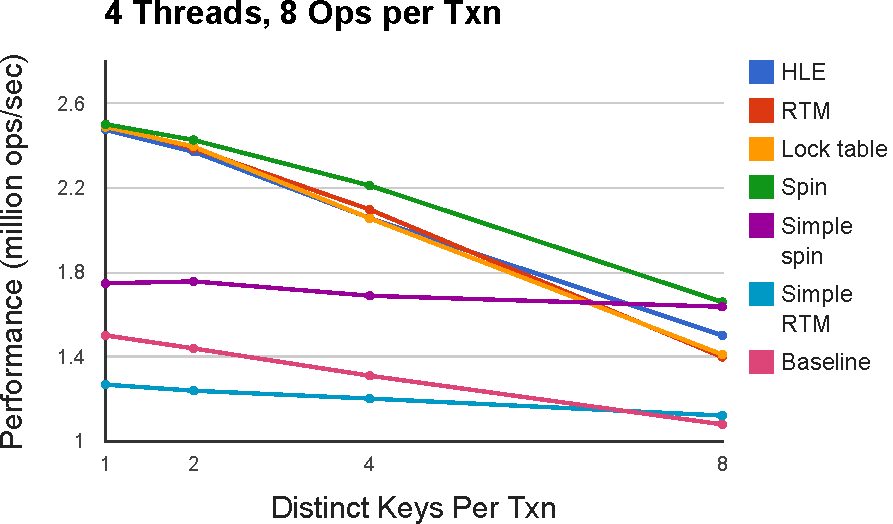
\includegraphics[scale=0.575]{figure/small_txns.pdf}
  \caption{Effect on different schemes of varying contention, using small
    transactions.}
  \label{fig:small_txns} 
\end{figure}

The results of varying contention when using small transaction sizes are shown
in \Cref{fig:small_txns}. For this experiment, we used transactions that
performed 8 operations on the hashtable, while varying the number of distinct
keys that each transaction touches from 1 to 8. The data reflects 4 running
threads, which we found to be the ``sweet spot'' for generating a large enough
workload to saturate the CPU without overwhelming it. The baseline is an
exception: it was run single-threaded and without any concurrency control.

As the graph shows, the baseline implementation is relatively unaffected by the
increase in contention -- it is single threaded, so it never has to stop
transactions to wait for another to complete. The slight drop in performance is
due to the increased amount of time that it takes to generate transactions with
a large number of keys.

The simple spin lock implementation is similarly unaffected by increased
contention, because it grabs a single lock for the entire table for each
transaction regardless of the keys in the transaction. This scheme achieves a
higher throughput than the baseline implementation, and is also less affected by
increases in contention. This is because per-transaction overheads, such as
the generation of the keys each transaction will touch, are not performed in the
lock's critical section, allowing for a very small degree of parallelism that
the baseline implementation does not have.

The worst performace is achieved by the simple RTM scheme, which aborts
essentially every transaction due its na\"{\i}ve use of hardware transactional
memory.  As a result, it falls back to using a single lock to protect the entire
table on every transaction. This leads to performance that does not degrade with
increased contention -- exactly like the simple spin lock's, but with
significantly lower throughput due to time spent aborting and retrying
transactions.

All of the other schemes are fine-grained to increase concurrency, and as a
result their performance degrades as contention is increased.

The hardware schemes do not perform any better than the software schemes. We
believe that this is because there are two competing effects at work. On the one
hand, locks are sometimes successfully elided and transactions are able to
complete successfully without interference. In this case, the HTM schemes are
faster than the software schemes, which never elide locks.  However, if a
conflict causes HTM to abort, it must re-execute the transaction, making it
slower than the software methods. When the maximum number of aborts before
locking the entire table is configured optimally for the hardware schemes, these
factors roughly cancel each other out. This also accounts for the greater drop
in performance of the hardware-based schemes as contention increases, since
greater contention leads to more aborts.

A final takeaway from this graph is that the performance of fine-grained spin
locks is better than that of the fine-grained lock table under high contention,
presumably because spin locks impose less overhead. In particular, spin locks do
not force the many context switches that a lock table causes by sleeping and
waking threads for each conflict.

\begin{figure}[h!]
  \centering
  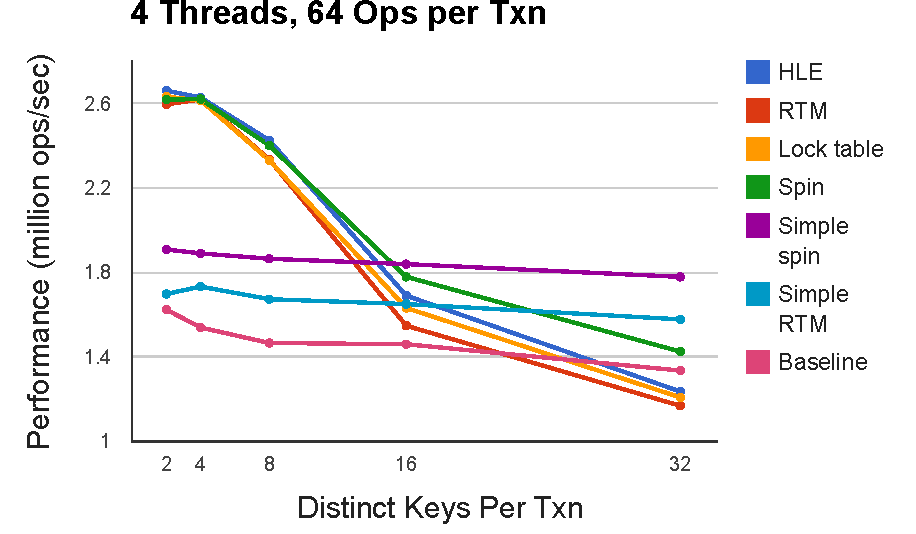
\includegraphics[scale=0.575]{figure/large_txns.pdf}
  \caption{Effect on different schemes of varying contention, using large
    transactions.}
  \label{fig:large_txns} 
\end{figure}

We also wanted to measure the effects of increased contention while using a
large transaction size. The results of this experiment are reflected in
\Cref{fig:large_txns}. For this experiment, we used transactions that performed
64 hashtable operations, and varied the number of distinct keys in each
transaction from 2 to 32. As with the small transactions, results reflect
running with 4 threads, except for the baseline which uses one thread.

As expected, the shape of the different schemes' performance follows the same
pattern as for the experiment with small transactions. The peak throughput here
is somewhat higher -- over 2.6 million, versus about 2.5 million for small
transactions. This is because each transaction performs more work, so there is
less of a slowdown from per-transaction overheads such as passing the
transaction to the transaction manager. Despite the significant increase in
transaction size, this effect is small because most of the per-transaction
overhead, such as generating keys for the transaction, increases with more
operations per transaction.

It is also noteworthy that the performance of the fine-grained schemes degrades
much more dramatically here than in the small transactions experiment. This is
partially due to a much longer per-transaction critical section, which results
in longer lock waits in the lock-based schemes and more aborts in the
hardware-based schemes. Another cause is the fact that this experiment achieves
much higher contention than the small-transaction test. Our hashtable contains
only $2^{14}$ keys, and the Zipfian distribution of key accesses produces a
large number of accesses to a small number of ``hot'' keys. With up to 4
transactions attempting to run simultaneously, if each transaction touches 32
distinct keys, the probability of each transaction conflicting with another is
extremely high.

In fact, as the graph demonstrates, when the contention becomes high enough it
is actually more efficient to use a simple spin lock than one of the more
sophisticated schemes. This is because fine-grained locking adds a large amount
of overhead, and in the case of very high contention adds little to the
potential concurrency of the system.

\subsection{Varying Threads}

Another effect that we wished to study is the performance of the different
schemes under heavier and lighter workloads. We determined the intensity of the
workload by varying the number of threads concurrently accessing the hash
table. (The baseline was again run for a single thread, this time with its
results averaged over 9 runs.)

\begin{figure}[h!]
  \centering
  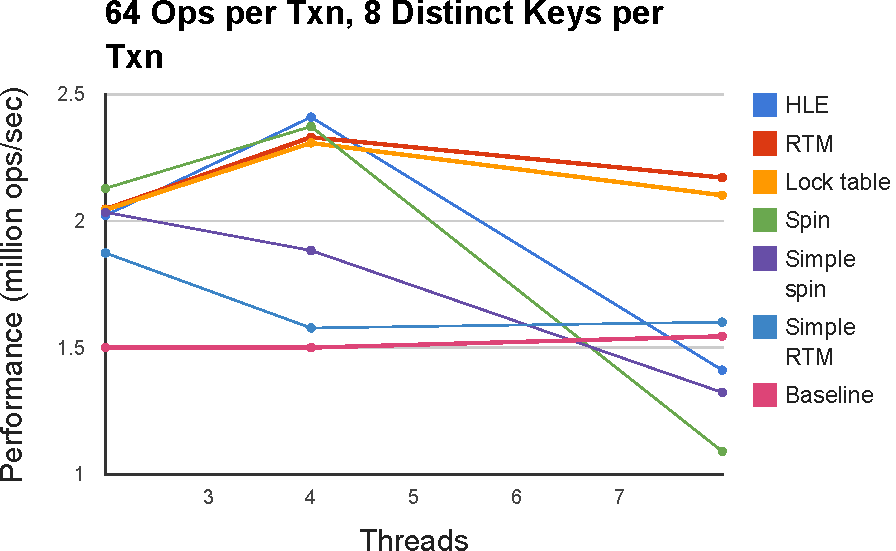
\includegraphics[scale=0.575]{figure/threads.pdf}
  \caption{Effect on different schemes of varying the number of threads.}
  \label{fig:threads} 
\end{figure}

The results of this experiment as shown in \Cref{fig:threads}. In this
experiment, we varied the number of threads from 2 to 8. We used large
transactions (64 operations each) and a moderate level of contention, with each
transaction working on 8 distinct keys.

As expected, most of the schemes follow the pattern of initially increasing in
performace, peaking at around 4 threads, and then declining with increasing
threads. This is because a very small number of threads does not take advantage
of all of the potential parallelism, resulting in lower throughput, whereas a
very large number of threads results in too much contention and degrades
performance as a result.

When we varied contention for a single workload (see \Cref{fig:large_txns}), the
fine-grained spin lock implementation performed better than the lock table
implementation. Increasing the workload size gives the opposite result. This
results from contention for CPU resources: spin locks suffer because they impose
a constant load on the CPU, whereas the lock table simply puts threads to sleep
while they are waiting on a lock to become free. This allows the lock table to
handle a high number of threads more gracefully.

It is also noteworthy that RTM's performance is similar to that of the lock
table's, whereas HLE's performance more closely matches that of the fine-grained
spin locks.  This is because the fallback path for HLE is to grab a 
spin lock, whereas the fallback path for RTM was configured to use a 
mutex, like the locks in the lock table.

The other schemes do not follow this same pattern of increasing then decreasing
performance. In particular, the simple spin lock scheme does not show any
increase in performace, as it only allows a single transaction to execute at a
time regardless of the number of threads.

\subsection{Dynamic Read/Write Sets}

The final experiment that we ran measured the effects of dynamic read/write sets
on the different concurrency control methods. This is significant because it
leads to the possibility of deadlock, which we avoided in the previous
experiment by enforcing an ordering in which the locks would be grabbed by the
fine-grained schemes.

For this experiment, we reused the parameters from the second experiment:
large transactions of 64 operations, 4 running threads, and varying 
contention by increasing the number of distinct keys for each transaction 
from 2 to 32.

\begin{figure}[h!]
  \centering
  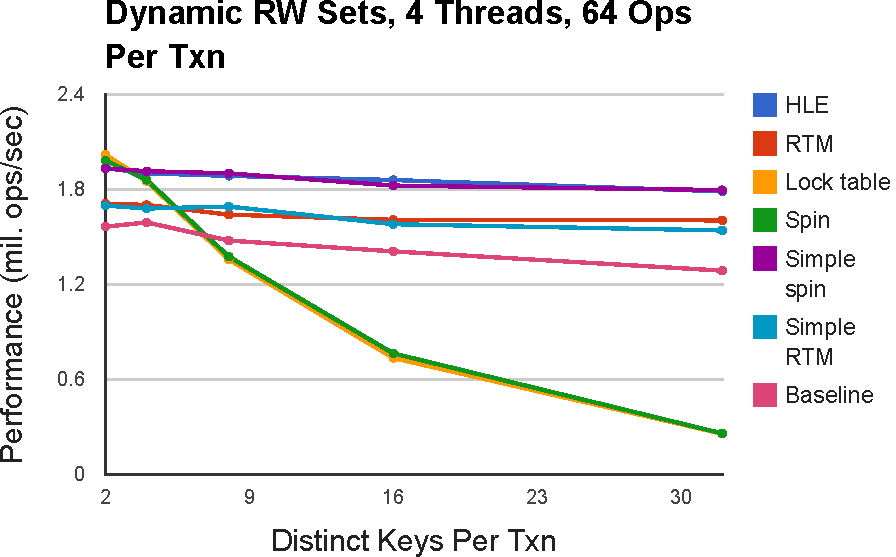
\includegraphics[scale=0.575]{figure/dynamic.pdf}
  \caption{Effect of dynamic read/write sets.}
  \label{fig:dynamic} 
\end{figure}

As \Cref{fig:dynamic} reflects, dynamic read/write sets have a dramatic impact
on the performance of the software-based schemes, resulting from the possibility
of deadlocks. We deal with deadlocks by timing out transactions that have been
waiting on a lock too long and aborting them. As contention increases, the
number of aborts becomes very high, dramatically reducing the throughput by more
than a factor of 2.

In contrast, the performance of the hardware-based schemes is unaffected by 
the dynamic read/write sets. This is because the only time these schemes 
actually grab a lock is in the fallback path, in which case there is only a 
single lock for the entire table and therefore no possibility of deadlock.

Admittedly, our deadlock prevention method is rather simple, and a more
sophisticated approach could offer better performance. However, implementing an
algorithm such as deadlock detection through dependency graphs is difficult and
complicated, and the hardware-based schemes are able to give good performance in
the face of dynamic read/write sets while still keeping the code simple.


